\chapter{Scalars: Spin 0 Fields}
\section{Deducing Klein-Gordon Equation}
If we squared the operators in the original Schrodinger equation, we obtain
\begin{equation}
\left(i \hbar \frac{\partial}{\partial t}\right)\left(i \hbar \frac{\partial}{\partial t}\right) \phi=H^{2} \phi=\left(\mathbf{p}_{o p e r}^{2} c^{2}+m^{2} c^{4}\right) \phi
\end{equation}
which becomes
\begin{equation}
-\frac{\hbar^{2}}{c^{2}} \frac{\partial^{2}}{\partial t^{2}} \phi=\left(-\hbar^{2} \frac{\partial}{\partial X_{i}} \frac{\partial}{\partial X_{i}}+m^{2} c^{2}\right) \phi
\end{equation}
In a compact form, we have
\begin{equation}
-\frac{\partial}{\partial x^{0}} \frac{\partial}{\partial x_{0}} \phi=\left(\frac{\partial}{\partial x^{i}} \frac{\partial}{\partial x_{i}}+\frac{m^{2} c^{2}}{\hbar^{2}}\right) \phi
\end{equation}
where we define $\mu^2=\frac{m^{2} c^{2}}{\hbar^{2}}$. Re-arranging, we have the Klein-Gordon equation
\begin{qt}
    \begin{equation}
\left(\partial_{\mu} \partial^{\mu}+\mu^{2}\right) \phi=0
\end{equation}
The operation $\partial_{\mu} \partial^{\mu}=\partial^{\mu} \partial_{\mu}$ is called the \textbf{d'Alembertian} operator, and is the 4D Minkowski coordinates analogue of the 3D Laplacian operator of Cartesian coordinates.
\end{qt}
\subsection{The solutions to the Klein-Gordon Equation}
\begin{equation}
\phi(x)=\sum_{n=1}^{\infty} \frac{1}{\sqrt{2 V E_{n} / \hbar}}\left(A_{n} e^{-\frac{i}{\hbar}\left(E_{n} t-\mathbf{p}_{n} \cdot \mathbf{x}\right)}+\underbrace{B_{n}^{\dagger} e^{\frac{i}{\hbar}\left(E_{n} t-\mathbf{p}_{n} \cdot \mathbf{x}\right)}}_{\text {absent in NRQM }}\right)
\end{equation}
Because we are using the square of the relativistic Hamiltonian in RQM, \bluep{we get additional solutions of exponential form $+i(E_nt-\mathbf{p}_n\cdot\mathcal{x})/\hbar$ that also solve the relativistic Klein-Gordon equation}.

With an aim towards using natural units, we note the following relations, where wave number $k_{i}$ $=2 \pi / \lambda_{i}$ and we use the deBroglie relation $p^{i}=\hbar k^{i}$
\begin{qt}
    \begin{equation}
p_{\mu}=\left[\begin{array}{c}
{E / c} \\
{p_{i}}
\end{array}\right]=\left[\begin{array}{c}
{E / c} \\
{-p^{i}}
\end{array}\right]=\hbar k_{\mu}=\left[\begin{array}{c}
{\hbar \omega / c} \\
{-\hbar k^{\prime}}
\end{array}\right]
\end{equation}
in natural units
\begin{equation}
p_{\mu}=\left[\begin{array}{c}
{E} \\
{-p^{i}}
\end{array}\right]=k_{\mu}=\left[\begin{array}{c}
{\omega} \\
{-k^{i}}
\end{array}\right]
\end{equation}
\end{qt}
Recall the notation introduced in the previous chapter, we have
\begin{equation}
p x=p_{\mu} x^{\mu}=E t-p^{i} x^{i}=p^{\mu} x_{\mu}
\end{equation}
\begin{equation}
k x=k_{\mu} x^{\mu}=\omega t-k^{i} x^{i}=\frac{E t}{\hbar}-\frac{p^{i} x^{i}}{\hbar}=\frac{p_{\mu}}{\hbar} x^{\mu}
\end{equation}
In natural unit
\begin{equation}
E=\omega, \quad p_{i}=k_{i}, \quad p_{\mu}=k_{\mu}, \quad p x=k x
\end{equation}
\bluep{For free fields, a given wave with wave number vector $\mathbf{k}$ has a particular energy, and we can designate that energy via either $E_{\mathbf{k}} \text { or } \omega_{\mathbf{k}} .$ It is common practice for scalars to use $\mathbf{k} \text { (rather than } \mathbf{p})$ and $\mathbf{k}$ (rather than $E_{\mathbf{p}}$ or $E_{\mathbf{k}}$.)}

The Klein-Gordon equation solutions then become, in natural units
\begin{equation}
\phi(x)=\sum_{k} \frac{1}{\sqrt{2 V_{e l}}}\left(A_{k} e^{-i k x}+B_{k}^{\dagger} e^{i k x}\right)
\end{equation}
\begin{mybox}
In RQM, the solution $\phi$ is that of a general (sum of eigenstates) single particle state. Each eigenstate has mathematical form of
$$
\phi_{k, A}=\frac{e^{-i k x}}{\sqrt{V}}
$$
$$
\quad \phi_{\mathrm{k}, B^{\dagger}}=\frac{e^{i k x}}{\sqrt{V}}
$$
Each of these forms has what is called \textbf{unit norm}. That is, all such eigenstates are \textbf{orthonormal}:
\begin{equation}
\int \phi_{k, A}^{\dagger} \phi_{k^{\prime},A} d^{3} x=\frac{1}{V} \int e^{i k x} e^{-i k^{\prime} x} d^{3} x=\delta_{k k^{\prime}}
\label{orthonormal-integral}
\end{equation}
Similar relations exist for $\phi_{k, B^{\dagger}}$.
\end{mybox}

\subsection{Deducing probability density in RQM}
Starting from the Klein-Gordon equation, first post-multiply it by $\phi^{\dagger}$, then subtract the complex conjugate equation post-multiplied by $\phi$,
\begin{equation}
\begin{array}{c}
{\left\{\frac{\partial^{2}}{\partial t^{2}} \phi=\left(\nabla^{2}-\mu^{2}\right) \phi\right\} \phi^{\dagger}} \\
{-\left\{\frac{\partial^{2}}{\partial t^{2}} \phi^{\dagger}=\left(\nabla^{2}-\mu^{2}\right) \phi^{\dagger}\right\} \phi}
\end{array}
\end{equation}
Since $\mu^{2} \phi^{\dagger} \phi-\mu^{2} \phi \phi^{\dagger}=0$, we obtain
\begin{equation}
i \frac{\partial}{\partial t}\left(\frac{\partial \phi}{\partial t} \phi^{\dagger}-\frac{\partial \phi^{\dagger}}{\partial t} \phi\right)=i \nabla \cdot\left((\nabla \phi) \phi^{\dagger}-\left(\nabla \phi^{\dagger}\right) \phi\right)
\end{equation}
where probability density and the probability current for a Klein-Gordon particle are
\begin{qt}
    \begin{equation}
\rho=j^{0}=i\left(\frac{\partial \phi}{\partial t} \phi^{\dagger}-\frac{\partial \phi^{\dagger}}{\partial t} \phi\right)
\end{equation}
and
\begin{equation}
\mathbf{j}=-i\left((\nabla \phi) \phi^{\dagger}-\left(\nabla \phi^{\dagger}\right) \phi\right) \quad j^{i}=-i\left(\phi_{,i} \phi^{\dagger}-\phi_{, i}^{\dagger} \phi\right)=i\left(\phi^{,i} \phi^{\dagger}-\phi^{\dagger, i} \phi\right)
\end{equation}
\end{qt}
Now we can define the \redp{4-currents} as
\begin{equation}
j^{\mu}=\left[\begin{array}{l}
{\rho} \\
{\mathbf{j}}
\end{array}\right]=\left[\begin{array}{l}
{\rho} \\
{j^{i}}
\end{array}\right]=\left[\begin{array}{l}
{j^{0}} \\
{j^{i}}
\end{array}\right]=i\left(\phi^{\mu} \phi^{\dagger}-\phi^{\dagger,\mu} \phi\right)
\end{equation}
The \redp{4D continuity equation} is then
\begin{qt}
    \begin{equation}
\frac{\partial j^{\mu}}{\partial x^{\mu}}=\partial_{\mu} j^{\mu}=j^{\mu}{ }_{,\mu}=0
\label{4d-continuity-eq}
\end{equation}
\end{qt}
(\ref{4d-continuity-eq}) tells us the important fact that \bluep{the 4-divergence of the 4-current of any conserved quantity is zero}.

\bluep{The total probability of unity is a relativistic invariant. Further $A_{k}$ here are constants that do not vary with frame.}\redp{So the probability of  finding any particular state is also independent of what frame the measurements are taken in.}

\subsection{Negative Energies in RQM}
If we apply traditional Hamiltonian operator $H$ as $i\partial/\partial t$ to $\phi_{\mathbf{k},B^{\dagger}}$:
\begin{equation}
i \frac{\partial \phi_{\mathbf{k}, B^{\dagger}}}{\partial t}=i \frac{\partial}{\partial t} \frac{e^{i k x}}{\sqrt{V}}=-\omega_{\mathbf{k}} \frac{e^{i k x}}{\sqrt{V}}=-\omega_{\mathbf{k}} \phi_{\mathbf{k}, B^{\dagger}}=E_{\mathbf{k}, B^{\prime}} \phi_{\mathbf{k}, B^{+}}
\end{equation}
Since $\omega_{\mathbf{k}}$ is always a positive number, we have states with \redp{negative energies in RQM, and we need QFT to solve this dilemma}. 

\section{Klein-Gordon Equation in Quantum Field Theory}
The fundamental scalar wave equation of RQM, the Klein-Gordon equation, is also the fundamental scalar wave equation of QFT,\redp{except that $\phi$ therein is considered a field, instead of a state.}

\bluep{The word "field" in quantum theory refers to a quantity that is spread out in space, but also, importantly, as we will soon see, is an \textbf{operator} in QFT. More properly, it is called a \textbf{quantum field or an operator field}, though the short term field is far more common.}
\begin{mybox}
In QFT, 
\begin{center}
    $|\phi\rangle$ symbolizes a state (particle)

$\phi$ symbolizes a field (operator),

Klein-Gordon equation is called a \textbf{field equation}.
\end{center}
\end{mybox}
\subsection{From classical relativistic fields to QFT}
The classical \textbf{Lagrangian density for a free, real, relativisitc scalar field $\phi$} has form
\begin{equation}
\mathcal{L}_{0}^{0}=K\left(\partial_{\alpha} \phi \partial^{\alpha} \phi-\mu^{2} \phi \phi\right)=
K\left(\dot{\phi} \dot{\phi}-\underbrace{\partial_{i} \phi \partial_{i} \phi}_{\nabla \phi \cdot \nabla \phi}-\mu^{2} \phi \phi\right)
\label{classical-scalar-fields}
\end{equation}
where $\phi$, since it is a classical field, is real (not complex), $\mu$ is a constant to be determined by experiment, $K$ is an arbitrary constant, the superscript $0$ on $\mathcal{L}$ stands for scalar (with $\operatorname{spin} 0$ ), and the subscript "0" means free.

Using the Legendre transformation, we can readily use (\ref{classical-scalar-fields}) to find the Hamiltonian density, where $\pi_0^0$ is the field conjugate momentum:
\begin{equation}
\mathcal{H}_{0}^{0}=\pi_{0}^{0} \dot{\phi}-\mathcal{L}_{0}^{0}=\underbrace{\frac{\partial \mathcal{L}_{0}^{0}}{\partial \dot{\phi}} \dot{\phi}}_{2 K \dot{\phi}} -\mathcal{L}_{0}^{0}=K\left(\dot{\phi} \dot{\phi}+\nabla \phi \cdot \nabla \phi+\mu^{2} \phi \phi\right)
\label{classical-scalar-fields-hamil}
\end{equation}
\bluep{We know that in QM most meaningful things are complex, not real. So now we take \textbf{classical field as complex}}: \redp{$\phi$ is complex.} Choosing $K=1$, we obtain the \textbf{free, complex scalar field Lagrangian and Hamiltonian densities}:
\begin{qt}
    \begin{equation}
\mathcal{L}_{0}^{0}=\left(\partial_{\alpha} \phi^{\dagger} \partial^{\alpha} \phi-\mu^{2} \phi^{\dagger} \phi\right)=\left(\dot{\phi}^{\dagger} \dot{\phi}-\nabla \phi^{\dagger} \cdot \nabla \phi-\mu^{2} \phi^{\dagger} \phi\right)
\label{scalar-relativistic-lagrangian}
\end{equation}
\begin{equation}
\mathcal{H}_{0}^{0}=\frac{\partial \mathcal{L}_{0}^{0}}{\partial \dot{\phi}^{r}} \dot{\phi}^{r}-\mathcal{L}_{0}^{0}=\underbrace{\frac{\partial \mathcal{L}_{0}^{0}}{\partial \dot{\phi}}}_{\pi_{0}^{0}=\dot{\phi}^{\dagger}} + \underbrace{\frac{\partial \mathcal{L}_{0}^{0}}{\partial \dot{\phi}^{\dagger}}}_{\pi_{0}^{0}=\dot{\phi}} \dot{\phi}^{\dagger}-\mathcal{L}_{0}^{0}=\dot{\phi} \dot{\phi}^{\dagger}+\nabla \phi^{\dagger} \cdot \nabla \phi+\mu^{2} \phi^{\dagger} \phi
\label{scalar-relativistic-hamil}
\end{equation}
\end{qt}
where $\phi$ and $\phi^{\dagger}$ are considered separate fields in the summation over field types $r$. Now we are ready to \textbf{derive the Klein-Gordon field equation.} from \textbf{Euler-Lagrange field equation}:
\begin{equation}
\frac{\partial}{\partial x^{\mu}}\left(\frac{\partial \mathcal{L}}{\partial \phi_{, \mu}^{r}}\right)-\frac{\partial \mathcal{L}}{\partial \phi^{r}}=0
\end{equation}
Substituting the Lagrangian density (\ref{scalar-relativistic-lagrangian}), we obtain the Klein-Gordon equation for fields
\begin{qt}
    \begin{equation}
\begin{aligned}
&\left(\partial_{\mu} \partial^{\mu}+\mu^{2}\right) \phi=\left(\square^{2}+\mu^{2}\right) \phi=0\\
&\left(\partial_{\mu} \partial^{\mu}+\mu^{2}\right) \phi^{\dagger}=\left(\square^{2}+\mu^{2}\right) \phi^{\dagger}=0
\end{aligned}
\label{klein-gordon-field-eq}
\end{equation}
\end{qt}
The discrete palne wave solutions to (\ref{klein-gordon-field-eq}) are
\begin{qt}
    \begin{equation}
\begin{aligned}
\phi(x) &=\underbrace{\sum_{k} \frac{1}{\sqrt{2 V a_{k}}} a(k) e^{-i k x}}+\underbrace{\sum_{k} \frac{1}{\sqrt{2 V \omega_{k}}} b^{\dagger}(k) e^{i k x}} \\
&=\phi^{+} \quad+\quad \phi^{-}
\end{aligned}
\label{solution-klein-gordon-field-eq1}
\end{equation}
    \begin{equation}
\begin{aligned}
\phi(x) &=\underbrace{\sum_{k} \frac{1}{\sqrt{2 V a_{k}}} b(k) e^{-i k x}}+\underbrace{\sum_{k} \frac{1}{\sqrt{2 V \omega_{k}}} a^{\dagger}(k) e^{i k x}} \\
&=\phi^{\dagger+} \quad+\quad \phi^{\dagger-}
\end{aligned}
\label{solution-klein-gordon-field-eq2}
\end{equation}
\end{qt}
\redp{As we will see later, the lower case coefficients are operators}. The continuous plane wave solutions are
\begin{equation}
\phi(x)=\int \frac{d^{3} k}{\sqrt{2(2 \pi)^{3} \omega_{k}}} a(\mathbf{k}) e^{-i k x}+\int \frac{d^{3} k}{\sqrt{2(2 \pi)^{3} \omega_{k}}} b^{\dagger}(\mathbf{k}) e^{i k x}
\end{equation}
\begin{equation}
\phi^{\dagger}(x)=\int \frac{d^{3} k}{\sqrt{2(2 \pi)^{3} \omega_{\mathrm{k}}}} b(\mathrm{k}) e^{-i k x}+\int \frac{d^{3} k}{\sqrt{2(2 \pi)^{3} \omega_{\mathrm{k}}}} a^{\dagger}(\mathrm{k}) e^{i k x}
\end{equation}

\section{Commutation Relations: The Crux of QFT}
Of overriding importance in the theory, as we will see, are the following coefficient commutation relations, which we will derive below from the $2^{\text {nd }}$ quantization postulate of (\ref{2nd-quantization-commutator}).
\begin{qt}
    \begin{equation}
\left[a(\mathbf{k}), a^{\dagger}\left(\mathbf{k}^{\prime}\right)\right]=\left[b(\mathbf{k}), b^{\dagger}\left(\mathbf{k}^{\prime}\right)\right]=\delta_{\mathbf{k} \mathbf{k}^{\prime}}(\text { discrete }) ; =\delta\left(\mathbf{k}-\mathbf{k}^{\prime}\right) \text { (continuous) }
\label{coefficient-commutator-klain-gordon-solution}
\end{equation}
The form of this relation tells us that $a(\mathbf{k})$ and $b(\mathbf{k})$ are operators.
\end{qt}
\subsubsection{Proof of coefficient commutation relations}
Starting from (\ref{2nd-quantization-commutator}), we take different spatial coordiantes, but the same time coordinate $t$ for $\phi$ and $\pi^0{ }_0$:
\begin{equation}
\left[\phi(\mathbf{x}, t) \pi_{0}^{0}(\mathbf{y}, t)-\pi_{0}^{0}(\mathbf{y}, t) \phi(\mathbf{x}, t)\right]=\left[ \phi(x, t) \dot{\phi}^{\dagger}(y, t)-\dot{\phi}^{\dagger}(y, t) \phi(x, t)\right]=i \delta(x-y)
\label{2nd-quantization-commutator-same-t}
\end{equation}
Plugging the discrete solutions into the middle part, we get
$$
\sum_{\mathbf{k}} \sum_{\mathbf{k}^{\prime}} \frac{i \omega_{\mathbf{k}}}{2 V \sqrt{\omega_{\mathbf{k}} \omega_{\mathbf{k}}}}\left(\begin{array}{c}
     -a_{\mathbf{k}} b_{\mathbf{k}^{\prime}} e^{-i\left(\omega_{\mathbf{k}}+\omega_{\mathbf{k}^{\prime}}\right) t} e^{i\left(\mathbf{k} \cdot \mathbf{x}+\mathbf{k}^{\prime} \cdot \mathbf{y}\right)}+a_{\mathbf{k}} a_{\mathbf{k}^{\prime}}^{\dagger} e^{-i\left(\omega_{\mathbf{k}}-\omega_{\mathbf{k}^{\prime}}\right) t} e^{i\left(\mathbf{k} \cdot \mathbf{x}-\mathbf{k}^{\prime} \cdot \mathbf{y}\right)}\\
     -b_{\mathbf{k}}^{\dagger} b_{\mathbf{k}^{\prime}} e^{i\left(\omega_{\mathbf{k}}-\alpha_{\mathbf{k}^{\prime}}\right) t} e^{-i\left(\mathbf{k} \cdot \mathbf{x}-\mathbf{k}^{\prime} \cdot \mathbf{y}\right)}+b_{\mathbf{k}}^{\dagger} a_{\mathbf{k}^{\prime}}^{\dagger} e^{i\left(\omega_{\mathbf{k}}+\omega_{\mathbf{k}^{\prime}}\right) t} e^{-i\left(\mathbf{k} \cdot \mathbf{x}+\mathbf{k}^{\prime} \cdot \mathbf{y}\right)}\\ 
     +b_{\mathbf{k}^{\prime}} a_{\mathbf{k}} e^{-i\left(\omega_{\mathbf{k}}+\omega_{\mathbf{k}^{\prime}}\right) t} e^{i\left(\mathbf{k} \cdot \mathbf{x}+\mathbf{k}^{\prime} \cdot \mathbf{y}\right)}+b_{\mathbf{k}^{\prime}} b_{\mathbf{k}}^{\dagger} e^{i\left(\omega_{\mathbf{k}}-\omega_{\mathbf{k}^{\prime}}\right) t} e^{-i\left(\mathbf{k} \cdot \mathbf{x}-\mathbf{k}^{\prime} \cdot \mathbf{y}\right)}\\
     -a_{\mathbf{k}^{\prime}}^{\dagger} a_{\mathbf{k}} e^{-i\left(\omega_{\mathbf{k}}-\omega_{\mathbf{k}^{\prime}}\right) t} e^{i\left(\mathbf{k} \cdot \mathbf{x}-\mathbf{k}^{\prime} \cdot \mathbf{y}\right)}-a_{\mathbf{k}^{\prime}}^{\dagger} b_{\mathbf{k}}^{\dagger} e^{i\left(\omega_{\mathbf{k}}+\omega_{\mathbf{k}^{\prime}}\right) t} e^{-i\left(\mathbf{k} \cdot \mathbf{x}+\mathbf{k}^{\prime} \cdot \mathbf{y}\right)}
\end{array}\right)
$$
Using the math identity for the 3D Dirac delta function:
\begin{equation}
\delta(\mathbf{x}-\mathbf{y})=\frac{1}{V} \sum_{n=-\infty}^{+\infty} e^{-i \mathbf{k}_{n} \cdot(\mathbf{x}-\mathbf{y})}
\label{3D-dirac-idneityt}
\end{equation}
and matching terms, we see \bluep{that all terms where $\mathbf{k}^{}\prime\neq \pm \mathbf{k}$ must equal zero since the identity (\ref{3D-dirac-idneityt}) has no terms in $\mathbf{k}$ and $\mathbf{k}^{\prime}$.} The remaining terms all have $k'=\pm k$ which means $\omega_{k}=\omega_{k^{\prime}}$.Some of these have an exponential form $i\left(\omega_{\mathbf{k}}+\omega_{\mathbf{k}}\right) t.$, and those terms give us a summation of terms over $\mathbf{k} $having form, for each possible $\mathbf{k}^{\prime}$, of
$$
\underbrace{\left(b_{k} a_{k}-a_{k} b_{k}\right)}_{\text {must }=0}\underbrace{e^{-i 2 \omega_{k} t}}_{\neq 0} e^{i k \cdot(x+y)}
$$
$$
\underbrace{\left(b_{\mathbf{k}}^{\dagger} a_{\mathbf{k}}^{\dagger}-a_{\mathbf{k}}^{\dagger} b_{\mathbf{k}}^{\dagger}\right)}_{\text {must }=0} e^{i 2 \omega_{\mathbf{k}} t} e^{-i \mathbf{k} \cdot(\mathbf{x}+\mathbf{y})}
$$
$$
\underbrace{\left(b_{-k} a_{k}-a_{k} b_{-k}\right)}_{\text {must }=0} e^{-i 2 \omega_{k} t} e^{i k \cdot(x-y)}
$$
$$
\underbrace{\left(b_{\mathbf{k}}^{\dagger} a_{-\mathbf{k}}^{\dagger}-a_{-\mathbf{k}}^{\dagger} b_{\mathbf{k}}^{\dagger}\right)}_{\text {must }=0} e^{i 2 \alpha_{\mathbf{k}} t} e^{-i \mathbf{k} \cdot(\mathbf{x}-\mathbf{y})}
$$
i.e., all time dependent terms eqaul 0, as no time dependence on RHS of (\ref{2nd-quantization-commutator-same-t}). The remaining relevant terms are in the following forms
$$
\underbrace{\left(a_{\mathbf{k}} a_{\mathbf{k}}^{\dagger}-a_{\mathbf{k}}^{\dagger} a_{\mathbf{k}}\right)}_{\text {must }=1} \underbrace{e^{-i\left(\omega_{\mathbf{k}}-\omega_{\mathbf{k}}\right) t}}_{=1}e^{i \mathbf{k} \cdot(x-y)}
$$
$$
\underbrace{\left(a_{\mathbf{k}} a_{-\mathbf{k}}^{\dagger}-a_{-\mathbf{k}}^{\dagger} a_{\mathbf{k}}\right)}_{\text {must }=0} e^{i \mathbf{k} \cdot(\mathbf{x}+\mathbf{y})}
$$
$$
\underbrace{\left(b_{-k} b_{\mathbf{k}}^{\dagger}-b_{\mathbf{k}}^{\dagger} b_{-\mathbf{k}}\right)}_{\text {must }=0} e^{-i \mathbf{k} \cdot(x+y)}
$$
\section{The Hamiltonian in QFT}
For a free scalar field $\mathcal{H}=\mathcal{H}_{0}^{0}$, we have
$$
\begin{array}{c}
      H_{0}^{0}=\int \mathcal{H}_{0}^{0} d^{3} x=\int\left(\dot{\phi} \dot{\phi}^{\dagger}+\nabla \phi^{\dagger} \cdot \nabla \phi+\mu^{2} \phi^{\dagger} \phi\right) d^{3} x= \\
     \int\left(\sum_{\mathbf{k}} \frac{\partial}{\partial t} \frac{1}{\sqrt{2 V \omega_{\mathbf{k}}}}\left(a(\mathbf{k}) e^{-i k x}+b^{\dagger}(\mathbf{k}) e^{i k x}\right)\right)\left(\sum_{\mathbf{k}^{\prime}} \frac{\partial}{\partial t} \frac{1}{\sqrt{2 V \omega_{\mathbf{k}^{\prime}}}}\left(b\left(\mathbf{k}^{\prime}\right) e^{-i k^{\prime} x}+a^{\dagger}\left(\mathbf{k}^{\prime}\right) e^{i k x}\right)\right) d^{3} x\\
     +\int\left(-\partial_{i} \phi^{\dagger} \partial^{i} \phi+\mu^{2} \phi^{\dagger} \phi\right) d^{3} x
\end{array}
$$
Expand the middle line here. All terms in the integration result in zero except when $\mathbf{k}^{\prime}=\mathbf{k}$ or $\mathbf{k}^{\prime}=-\mathbf{k}$, because we are integrating orthogonal functions between their boundaries. Also, because of (\ref{orthonormal-integral}), \bluep{the integral over $a(n) b(k) e^{-2i k x}, b^{\dagger}(k) a^{\dagger}(k) e^{2 i k x}$,$-a(x) a^{\dagger}(-k) e^{-i k x} e^{i(-k) x}$, and $-b^{\dagger}(k) b(-k) e^{i k x} e^{-i(-k) x}$ are zeros too}. Since the volume of integration above equals $V$, we end up with
\begin{equation}
\begin{aligned}
\int \dot{\phi} \dot{\phi}^{\dagger} d^{3} x &=\sum_{\mathbf{k}} \frac{\omega_{\mathbf{k}}}{2}\left(-a(\mathbf{k}) b(-\mathbf{k}) e^{-2 i \omega_{\mathbf{k}} t}+a(\mathbf{k}) a^{\dagger}(\mathbf{k})+b^{\dagger}(\mathbf{k}) b(\mathbf{k})-b^{\dagger}(\mathbf{k}) a^{\dagger}(-\mathbf{k}) e^{2 i \omega_{\mathbf{u}} t}\right) \\
&=\sum_{\mathbf{k}} \frac{\left(\omega_{\mathbf{k}}\right)^{2}}{2 \omega_{\mathbf{k}}}\left(-a(-\mathbf{k}) b(\mathbf{k}) e^{-2 i \omega_{\mathbf{k}} t}+a(\mathbf{k}) a^{\dagger}(\mathbf{k})+b^{\dagger}(\mathbf{k}) b(\mathbf{k})-b^{\dagger}(-\mathbf{k}) a^{\dagger}(\mathbf{k}) e^{2 i \omega_{\mathbf{k}} t}\right)
\end{aligned}
\end{equation}
Following similar steps we get
$$
\begin{array}{c}
     -\int \partial_{i} \phi^{\dagger} \partial^{i} \phi d^{3} x=\int \partial_{i} \phi^{\dagger} \partial_{i} \phi d^{3} x\\
     =\sum_{k} \frac{k^{2}}{2 \omega_{k}}\left(b(k) a(-k) e^{-2 i \omega_k t}+a^{\dagger}(k) a(k)+b(k) b^{\dagger}(k)+a^{\dagger}(k) b^{\dagger}(-k) e^{2i \omega_k t}\right)
\end{array}
$$
and
$$
\int \mu^{2} \phi^{\dagger} \phi d^{3} x=\sum_{\mathbf{k}} \frac{\mu^{2}}{2 \omega_{\mathbf{k}}}\left(b(\mathbf{k}) a(-\mathbf{k}) e^{-2 i\omega_kt}+b(\mathbf{k}) b^{\dagger}(\mathbf{k})+a^{\dagger}(\mathbf{k}) a(\mathbf{k})+a^{\dagger}(\mathbf{k}) b^{\dagger}(-\mathbf{k}) e^{2 i \omega_{\mathbf{k}} t}\right)
$$
Adding the final parts of the equations above, and using \redp{$\mathbf{k}^{2}+\mu^{2}=\left(\omega_{\mathrm{k}}\right)^{2}$} along with the coefficient commutation relations, we end up with
\begin{equation}
\begin{aligned}
H_{0}^{0} &=\sum_{\mathbf{k}} \frac{\omega_{\mathbf{k}}}{2}\left(\underbrace{a(\mathbf{k}) a^{\dagger}(\mathbf{k})}_{\text {use commutator }}+a^{\dagger}(\mathbf{k}) a(\mathbf{k})+b^{\dagger}(\mathbf{k}) b(\mathbf{k})+\underbrace{b(\mathbf{k}) b^{\dagger}(\mathbf{k})}_{\text {use commutator }}\right) \\
&=\sum_{\mathbf{k}} \omega_{\mathbf{k}}\left(a^{\dagger}(\mathbf{k}) a(\mathbf{k})+\frac{1}{2}+b^{\dagger}(\mathbf{k}) b(\mathbf{k})+\frac{1}{2}\right)
\end{aligned}
\end{equation}
or simply
\begin{qt}
    \begin{equation}
H_{0}^{0}=\sum_{\mathbf{k}} \omega_{\mathbf{k}}\left(N_{a}(\mathbf{k})+\frac{1}{2}+N_{b}(\mathbf{k})+\frac{1}{2}\right)
\end{equation}
where
\begin{equation}
N_{a}(\mathbf{k})=a^{\dagger}(\mathbf{k}) a(\mathbf{k}) \quad N_{b}(\mathbf{k})=b^{\dagger}(\mathbf{k}) b(\mathbf{k})
\end{equation}
$\underline{N}_{a}(\mathbf{k})=$ number operator with eigenvalue $n_{a}(\mathbf{k})=$ number of $a$ particles with $3-$ mom $\mathbf{k}$ in the ket, 

$\underline{N}_{b}(\mathbf{k})=$ number operator with eigenvalue $n_{b}(\mathbf{k})=$ number of $b$ particles with 3 -mom $\mathbf{k}$ in the ket, 

and, the vacuum has $1 / 2$ quantum of energy for each $\mathbf{k}$ for $a$ particles, and also for $b$ particles.
\end{qt}
\bluep{We also anticipate that the $b$ type particles will be antiparticles, and the $a$ types, normal particles.}
\begin{example}
10 particle state
$$
H_{0}^{0}|5\phi_{k_{1}},2 \phi_{k_{2}},\underbrace{3 \bar{\phi}_{k_{3}}}_{b \text { type } \text { particles }}\rangle$$
$$=\sum_{k} \omega_{k}\left(N_{a}(k)+\frac{1}{2}+N_{b}(k)+\frac{1}{2}\right)| 5 \phi_{k_{1}}, 2 \phi_{k_{2}}, 3 \bar{\phi}_{k_{3}}\rangle
$$
$$
=\left(5 \omega_{\mathrm{k}_{1}}+2 \omega_{\mathrm{k}_{2}}+3 \omega_{\mathrm{k}_{3}}+\sum_{\mathrm{k}} \omega_{\mathrm{k}}\left(\frac{1}{2}+\frac{1}{2}\right)\right)\left(5 \phi_{\mathrm{k}_{1}}, 2 \phi_{\mathrm{k}_{2}}, 3 \bar{\phi}_{\mathrm{k}_{3}}\right)
$$
Vaccum state
$$
H_{0}^{0} \underbrace{| 0\rangle}_{\text {vacuum } \text { state }}=\sum_{\mathbf{k}} \omega_{\mathbf{k}}\left(N_{a}(\mathbf{k})+\frac{1}{2}+N_{b}(\mathbf{k})+\frac{1}{2}\right)|0\rangle
$$
$$
=
\underbrace{\sum_{\mathbf{k}} \omega_{\mathbf{k}}\left(\frac{1}{2}+\frac{1}{2}\right)}_{\text {infinite energy }}|0\rangle
$$
\end{example}
\subsection{Unit Nors and Orthogonality for Multiparticle States}
\begin{equation}
\begin{aligned}
&\left\langle\phi_{k}|| \phi_{k}\right\rangle=\int_{V} \underbrace{\phi_{k}^{\dagger}(x, t) \phi_{k}(x, t)}_{\text {slates }} d^{3} x=1
\end{aligned}
\end{equation}
\begin{equation}
\left\langle\phi_{\mathbf{k}} \| \phi_{\mathbf{k}^{\prime}}\right\rangle=\int_{V} \underbrace{\phi_{\mathbf{k}}^{\dagger}(\mathbf{x}, t) \phi_{\mathbf{k}^{\prime}}(\mathbf{x}, t)}_{\text {states }} d^{3} x=0, \mathbf{k} \neq \mathbf{k}^{\prime}
\end{equation}
\textbf{Note}: It is assumed that the ket is expressed in the position basis. The ket symbol $|\phi\rangle$ in general represents a particle state, but the form of the ket when we write it out mathematically changes with the basis we care to use for eyample. For example, we could express the ket in the momentum basis (in momentim space) instead of the position basis $x ;$ or in a number of other ways. Mathematically, 
$$
\left|\phi_{\mathbf{k}}\right\rangle= A e^{-i(E t-\mathbf{k} \cdot \mathbf{x})} \quad\left(\left|\phi_{\mathbf{k}}\right\rangle \text { here is expressed in the position basis }\right)
$$
is really $|\phi\rangle_{x \text { basis }}=\langle x | \phi\rangle= A e^{-i(E t-k \cdot x)}$

\section{Creation and Destruction Operators}
\textbf{Proof that $a(\mathrm{k})$ is a Particle Destruction Operator}

What can we say about the state
$$
a(\mathbf{k})\left|n_{\mathbf{k}}\right\rangle=\left|m_{\mathbf{k}}\right\rangle
$$
To see this, first operate on this state with our number operator
$$
N_{a}(\mathbf{k})\left|m_{\mathbf{k}}\right\rangle= N_{a}(\mathbf{k}) a(\mathbf{k})\left|n_{\mathbf{k}}\right\rangle=\underbrace{a^{\dagger}(\mathbf{k}) a(\mathbf{k})}_{\text {use commuttor }} a(\mathbf{k})\left|n_{\mathbf{k}}\right\rangle
$$
Then we use the commutation relations:

$\left(a(k) a^{\dagger}(k)-1\right) a(k)\left|n_{k}\right\rangle= a(k) a^{\dagger}(k) a(k)\left|n_{k}\right\rangle- a(k)\left|n_{k}\right\rangle= a(k) N_{a}(k)\left|n_{k}\right\rangle- a(k)\left|n_{k}\right\rangle=$

$= a(k) n_{k}\left|n_{k}\right\rangle- a(k)\left|n_{k}\right\rangle= n_{k} a(k)\left|n_{k}\right\rangle- a(k)\left|n_{k}\right\rangle=\left(n_{k}-1\right) a(k)\left|n_{k}\right\rangle=\left(n_{k}-1\right)\left|m_{k}\right\rangle$
So
$$
N_{a}(\mathrm{k})\left|m_{\mathrm{k}}\right\rangle=\left(n_{\mathrm{k}}-1\right)\left|m_{\mathrm{k}}\right\rangle= m_{\mathrm{k}}\left|m_{\mathrm{k}}\right\rangle
$$
$$
m_{k}=n_{k}-1
$$
Similarly, we have

$\left.N_{a}(\mathrm{k})\left(a(\mathrm{k}) | n_{\mathrm{k}}\right)\right\rangle=\left(n_{\mathrm{k}}-1\right)\left(a(\mathrm{k})\left|n_{\mathrm{k}}\right\rangle\right)$

$N_{a}(k)\left(a^{\dagger}(k)\left|n_{k}\right\rangle\right)=\left(n_{k}+1\right)\left(a^{\dagger}(k)\left|n_{k}\right\rangle\right.$

$N_{b}(k)\left(b(k)\left|\bar{n}_{k}\right\rangle\right)=\left(\bar{n}_{k}-1\right)\left(b(k)\left|\bar{n}_{k}\right\rangle\right)$

$N_{b}(k)\left(b^{+}(k)\left|\bar{n}_{k}\right\rangle\right)=\left(\bar{n}_{k}+1\right)\left(b^{+}(k)\left|\bar{n}_{k}\right\rangle\right)$

\redp{$a(k),b(k)$ are called lowered operators and $a^{\dagger}(k),b^{\dagger}(k)$ are called raised operators.}
\subsection{Normalization factors for raised and lowered states}
Consider
$$
a^{\dagger}(\mathbf{k})\left|n_{\mathbf{k}}\right\rangle= A\left|n_{\mathbf{k}}+1\right\rangle
$$
$$
\left(A\left|n_{\mathrm{k}}+1\right\rangle\right)^{\dagger}=\left(a^{\dagger}(\mathbf{k})\left|n_{\mathbf{k}}\right\rangle\right)^{\dagger}=\left\langle n_{\mathbf{k}}\left|a(\mathbf{k})=\left\langle n_{\mathbf{k}}+1\right| A^{+}\right.\right.
$$
Note that
$$
\left\langle n_{\mathbf{k}}\left|a(\mathbf{k}) a^{\dagger}(\mathbf{k})\right| n_{\mathbf{k}}\right\rangle=\left\langle n_{\mathbf{k}}+1\left|A^{\dagger} A\right| n_{\mathbf{k}}+1\right\rangle= A^{\dagger} A\left\langle n_{\mathbf{k}}+1 \| n_{\mathbf{k}}+1\right\rangle= A^{\dagger} A
$$
Also
$$
\left\langle n_{\mathbf{k}}\left|\underbrace{a(\mathbf{k}) a^{\dagger}(\mathbf{k})}_{\text { use commutator }}\right| n_{\mathbf{k}}\right\rangle=\left\langle n_{\mathbf{k}}|\underbrace{a^{\dagger}(\mathbf{k}) a(\mathbf{k})}_{N_{a}(\mathbf{k})}+1| n_{\mathbf{k}}\right\rangle=\left\langle n_{\mathbf{k}}\left|n_{\mathbf{k}}+1\right| n_{\mathbf{k}}\right\rangle= n_{\mathbf{k}}+1
$$
Thus $A=\sqrt{n_{k}+1}$.
\begin{qt}
    \begin{equation}
\begin{aligned}
a^{\dagger}(\mathbf{k})\left|n_{\mathbf{k}}\right\rangle &=\sqrt{n_{\mathbf{k}}+1}\left|n_{\mathbf{k}}+1\right\rangle \\
a(\mathbf{k})\left|n_{\mathbf{k}}\right\rangle &=\sqrt{n_{\mathbf{k}}} | n_{\mathbf{k}}-1\rangle \\
b^{\dagger}(\mathbf{k})\left|\bar{n}_{\mathbf{k}}\right\rangle &=\sqrt{\bar{n}_{\mathbf{k}}+1}\left|\bar{n}_{\mathbf{k}}+1\right\rangle \\
b(\mathbf{k})\left|\bar{n}_{\mathbf{k}}\right\rangle &=\sqrt{\bar{n}_{\mathbf{k}}}\left|\bar{n}_{\mathbf{k}}-1\right\rangle
\end{aligned}
\end{equation}
\end{qt}
Note that \redp{a lowering operator destroys the vacuum state.} In summary, \bluep{second quantization turned the solution coefficient in RQM, which were merely constants, into creation and destruction operators in QFT.}

\subsection{Total Particle Number}
For future use, we define the \textbf{total particle number as the number of particles (i.e. a types) minus the number of antiparticles ( b types)}. For scalars, the total particle number operator is
\begin{equation}
    N(\phi)=\sum_{k}\left(N_{a}(\mathbf{k})-N_{b}(\mathbf{k})\right)
\end{equation}
\subsection{Operator Fields}
The total particle lowering operator field is
\begin{equation}
\phi=\underbrace{\phi^{+}}_{\text {destroys particles }}+\underbrace{\phi^{-}}_{\text {creates anti-particles}}
\end{equation}
The total particle raising operator field is
\begin{equation}
\phi^{\dagger}=\underbrace{\phi^{\dagger+}}_{\text {destroys anti-particles }}+\underbrace{\phi^{\dagger-}}_{\text {Creates particles}}
\end{equation}
\subsection{Normal Ordering}
One approach to solving \redp{"infinite vacuum energy" problem is called normal ordering.} \bluep{Normal ordering, in any term, consists of moving all destruction operators to the right-hand side of that term.} With this ordering, we have the Hamiltonian as:
\begin{equation}
H_{0}^{0}=\sum_{\mathbf{k}} \omega_{\mathbf{k}}\left(a^{\dagger}(\mathbf{k}) a(\mathbf{k})+b^{\dagger}(\mathbf{k}) b(\mathbf{k})\right)
\end{equation}
Note that normal ordering is often justified because particle/field behavior in our theories of classical mechanics, electromagnetism, and special relativity depends on energy difference, so we can take our reference as the vacuum energy level and all energies of interest are relative to that. In those theories, it is $\Delta E$ that is important, not $E .$ So, why not assume our Hamiltonian represents $\Delta E$ instead of $E ?$ The answer is because in general relativity, the theory depends on $E .$ To be consistent with all of physics, we need $H$ representing $E,$ not $\Delta E$.

\section{Probability, Four Currents, and Charge Density}
Since our governing equation is the Klein-Gordon equation, and tha is the same as in RQM, we can follow the similar steps to derive the same 4-current relations, except that $\phi$ and $\phi^{\dagger}$ are now operator fields:
\begin{qt}
    \begin{equation}
j^{\mu},_{\mu}=0 \text { with } j^{\mu}=i\left(\phi^{\mu} \phi^{\dagger}-\phi^{\dagger \mu} \phi\right) \quad j^{\mu} \text { is an operator }
\label{field-4-current}
\end{equation}
\begin{equation}
\rho=j^{0}=i\left(\frac{\partial \phi}{\partial t} \phi^{\dagger}-\frac{\partial \phi^{\dagger}}{\partial t} \phi\right)
\label{field-probability-density-operator}
\end{equation}
\end{qt}
Since (\ref{field-probability-density-operator}) is an operator, we \textbf{need its expectation value to find measurable probability density},
$$
\bar{\rho}=\left\langle\phi, \phi_{2}, \phi_{3}, \ldots|\rho| \phi, \phi_{2}, \phi_{3}, \ldots\right\rangle
$$
and
\begin{qt}
    \begin{equation}
        \rho=\frac{1}{V} \sum_{k}\left(a^{\dagger}(\mathrm{k}) a(\mathrm{k})-b^{\dagger}(\mathrm{k}) b(\mathrm{k})\right)=\frac{1}{V} \sum_{\mathrm{k}}\left(N_{a}(\mathrm{k})-N_{b}(\mathrm{k})\right)
    \end{equation}
\end{qt}
For single particle state
$$
\bar{\rho}=\left\langle\phi_{k}|\rho| \phi_{k}\right\rangle=\left\langle\phi_{k}\left|\frac{1}{V} \sum_{k}\left(N_{a}(k)-N_{b}(k)\right)\right| \phi_{k}\right\rangle=\left\langle\phi_{k}\left|\frac{1}{V}\right| \phi_{k}\right\rangle=\frac{1}{V}
$$
\bluep{For a plane wave, this is exactly our probability density, a flat distribution over the volume.}

For antiparticles(type b particles), we obtain \redp{negative probability}:
$$
\bar{\rho}=\left\langle\bar{\phi}_{\mathrm{k}}|\rho| \bar{\phi}_{\mathrm{k}}\right\rangle=\left\langle\bar{\phi}_{\mathbf{k}^{\prime}}\left|\frac{-1}{V}\right| \bar{\phi}_{\mathbf{k}^{\prime}}\right\rangle=-\frac{1}{V}
$$
\textbf{This was another tip to early researchers that the density here was more readily related to \redp{charge density}, and the b particles were antiparticles, with opposite charge and charge density from particles.}
\subsection{Charge density not probability density}
If we multiply our four current operator (\ref{field-4-current}) by the charge of a scalar particle $q$ it behaves like a charge density operator, which we will designate by $s^{\mu}$
\begin{qt}
    \begin{equation}
s_{\mu}^{\mu}=0 \quad \text { with } \quad s^{\mu}=q j^{\mu}=i q\left(\phi^{, \mu} \phi^{\dagger}-\phi^{\dagger,\mu}  \phi\right)
\end{equation}
So
\begin{equation}
\rho_{\text {charge }}=q^{0}=i q\left(\frac{\partial \phi}{\partial t} \phi^{\dagger}-\frac{\partial \phi^{\dagger}}{\partial t} \phi\right)
\end{equation}
\end{qt}
\subsection{Caution in evaluating expectation values of density operators}
\redp{For operators with a spatial dependence such as $\rho$ often has, the spatial dependence in the operator is not included in the integration.} That is. writing out the expectation values as an integral, we integrate over the $\mathbf{x}^{\prime}$ of the state, but not the $\mathbf{x}$ of the operator:
\begin{equation}
\langle\rho(\mathbf{x}, t)\rangle=\left\langle\phi_{\mathbf{k}}\left(\mathbf{x}^{\prime}, t\right)|\rho(\mathbf{x}, t)| \phi_{\mathbf{k}}\left(\mathbf{x}^{\prime}, t\right)\right\rangle=\int \phi_{\mathbf{k}, \text { state }}^{\dagger}\left(\mathbf{x}^{\prime}, t\right) \rho(\mathbf{x}, t) \phi_{\mathbf{k}, \text {state}}\left(\mathbf{x}^{\prime}, t\right) d^{3} x^{\prime}
\end{equation}

\subsection{Charge operator}
Regarding charge, we need merely to integrate our charge density operator $qj^0$ over the entire volume, to get the \textbf{charge operator}:
\begin{equation}
Q=\int s^{0} d^{3} x=q \int j^{0} d^{3} x=q \sum_{\mathbf{k}}\left(N_{a}(\mathbf{k})-N_{b}(\mathbf{k})\right)
\end{equation}

\subsection{Three momentum operator}
\begin{equation}
p^{\prime}=\int  \mathcal{R}^{i} d^{3} x=-\int \pi_{r} \frac{\partial \phi^{r}}{\partial x^{i}} d^{3} x=-\int\left(\frac{\partial \mathcal{L}}{\partial \dot{\phi}} \frac{\partial \phi}{\partial x^{i}}+\frac{\partial \mathcal{L}}{\partial \dot{\phi}^{\dagger}} \frac{\partial \phi^{\dagger}}{\partial x^{i}}\right) d^{3} x
\end{equation}
Substituting the Klein-Gordon solutions, we find
\begin{equation}
P=\sum_{k} k\left(N_{a}(k)+N_{b}(k)\right)
\end{equation}
\bluep{Similar to what happened to charge, we have 1/2 quanta in the vacuum with 3-momentum, but the total for the vacuum sums to zero. Unlike energy, this is a vector summation, and for every 3-momentum $\mathbf{k}$ in the sum, there is a 3-momentum $-\mathbf{k}$, as well.} The net is nil 3-momentum for the vacuum, which again, is a welcome result.

So far in our theory, only energy has proved problematic in having a non-zero vacuum expectation value (VEV).

\subsection{Four momentum operator}
\begin{equation}
\underbrace{P^{\mu}=K^{\mu}}_{\text {operators }}=\underbrace{\left(\begin{array}{l}
{H} \\
{\mathbf{p}}
\end{array}\right)}_{for free scalars}=\sum_{\mathbf{k}}\left(\begin{array}{c}
{\omega_{\mathbf{k}}} \\
{\mathbf{k}}
\end{array}\right)\left(N_{a}(\mathbf{k})+N_{b}(\mathbf{k})\right)
\end{equation}
where we note that $k^{\mu}$ usually refers to the numeric (not operator) 4 vector $(\omega_{ \mathbf{k}}, \mathbf{k})$

\subsection{Klein-Gordon states are Bosons}
Using the same scalar creation operator repeatedly on a state results in a raised state containing a number of the same particle with the same $\mathbf{k}$ (and thus the same energy and identical in all regards.) For example,

$$
a(k)^{\dagger}|0\rangle=\left|\phi_{k}\right\rangle\rightarrow a(\mathrm{k})^{\dagger}\left|\phi_{k}\right\rangle=\sqrt{2}\left|2 \phi_{k}\right\rangle\rightarrow a(\mathrm{k})^{+}\left|2 \phi_{\mathrm{k}}\right\rangle=\sqrt{3}\left|3 \phi_{\mathrm{k}}\right\rangle \rightarrow\dots
$$

This means Klein-Gordon states must be bosons.

\subsection{Other useful operators}
To \textbf{create a general single particle state}, we use the following creation operator:
\begin{equation}
C=\sum_{k} A_{k} a_{k}^{\dagger}
\end{equation}
For example,
$$
C|0\rangle=\sum_{\mathbf{k}} A_{\mathbf{k}} \mathbf{a}_{\mathbf{k}}^{\dagger}|0\rangle= A_{1}\left|\phi_{1}\right\rangle+ A_{2}\left|\phi_{2}\right\rangle+ A_{3}\left|\phi_{3}\right\rangle+\ldots=|\phi\rangle
$$
and
$$
\sum_{\mathbf{k}}\left|A_{\mathbf{k}}\right|^{2}=1
$$
Similarly, we can destroy a general single particle state using
\begin{equation}
D=\sum_{\mathbf{k}} \mathbf{a}_{\mathbf{k}}
\end{equation}
\begin{mybox}
\textbf{What $\phi(x)$ and $\phi^{\dagger}(x)$ Create When Acting on the Vacuum ?}

$\phi(x)$ acting on the vacuum will create a single general antiparticle state comprising superposition of an infinite number of eigenstates, each with a constant coefficient in front of it, i.e.,
$$
\phi(x)|0\rangle=\sum_{\mathbf{k}} \frac{1}{\sqrt{2 V \omega_{\mathbf{k}}}} e^{-i k x} \underbrace{a(\mathbf{k})|0\rangle}_{0}+\sum_{\mathbf{k}} \frac{1}{\sqrt{2 V a_{\mathbf{k}}}} e^{i k x} \underbrace{b^{\dagger}(\mathbf{k})|0\rangle}_{|\bar{\phi}_k\rangle}=\sum_{\mathbf{k}} \frac{1}{\sqrt{2 V \omega_{\mathbf{k}}}} \underbrace{e^{i k x}\left|\bar{\phi}_{\mathbf{k}}\right\rangle}
$$
\end{mybox}
\subsection{Fock space and Hilbert space}
In $\mathrm{NROM}$ and $\mathrm{RQM},$ the states are single particle states and the abstract space they inhabit is called \textbf{Hilbert space}, which has a different single particle eigenstate as the basis vector of each "axis'. The dimension of the Hilbert space for a given system is simply the number of linearly independent eigenstates in that system. This can, for many systems, be infinite.

The multiparticle abstract state space of $\mathrm{QFT}$ is called Fock space, which is simply an extension of Hilbert space to multiparticle states.

\subsection{a(k) Destroys Any State without Single a Type Particle in k Eigenstate}
\begin{example}
For a multi-particle state
$$
a_{2}\left|\phi_{1}, 4 \phi_{3}, 7 \bar{\phi}_{2}\right\rangle= 0
$$
\end{example}
In general, a particular type particle destruction operator of given $\mathbf{k}$ acting on a state that has no particles of that type of the same 3 -momentum k results in zero.

\section{Derive Scalar Feynman Propagator}
In the course of deriving the interaction theory, a mathematical relationship arises that is called the Feynman propagator. Physically, it can be visualized as repesenting a virtual particle that exists fleetingly and carries energy, momentum, and in some cases, charge from one real particle to another. \textbf{Thus, it is the carrier, or mediator, of force (interaction).}

\bluep{From a heuristic perspective the operator field $\phi^{\dagger}(y)$ can be considered to create a virtual scalar particle at event $y$, and the field operator $\phi(x)$ destroys that virtual particle at event $x$.}

The entire derivation is for continuous (not discrete) eigenstate solutions of the field equation (Klein-Gordon here), since the propagator represents a virtual particle in the vacuum and the vacuum is not confined to a volume $V$. We represent the scalar Feynman propagator with the symbol $i \Delta_{F}(x-y) .$ (Including the imaginary factor $i$ is common practice.)

\begin{figure}[H]
    \centering
\tikzset{every picture/.style={line width=0.75pt}} %set default line width to 0.75pt        

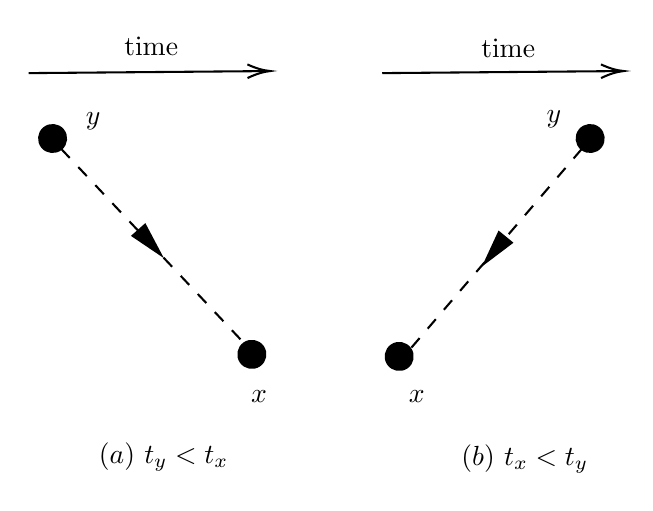
\begin{tikzpicture}[x=0.75pt,y=0.75pt,yscale=-1,xscale=1]
%uncomment if require: \path (0,300); %set diagram left start at 0, and has height of 300

%Straight Lines [id:da07703774414132791] 
\draw    (39,78) -- (153.33,77.02) ;
\draw [shift={(155.33,77)}, rotate = 539.51] [color={rgb, 255:red, 0; green, 0; blue, 0 }  ][line width=0.75]    (10.93,-3.29) .. controls (6.95,-1.4) and (3.31,-0.3) .. (0,0) .. controls (3.31,0.3) and (6.95,1.4) .. (10.93,3.29)   ;

%Straight Lines [id:da3375209545438721] 
\draw    (209.33,78) -- (323.67,77.02) ;
\draw [shift={(325.67,77)}, rotate = 539.51] [color={rgb, 255:red, 0; green, 0; blue, 0 }  ][line width=0.75]    (10.93,-3.29) .. controls (6.95,-1.4) and (3.31,-0.3) .. (0,0) .. controls (3.31,0.3) and (6.95,1.4) .. (10.93,3.29)   ;

%Shape: Circle [id:dp6041905468772015] 
\draw  [fill={rgb, 255:red, 0; green, 0; blue, 0 }  ,fill opacity=1 ] (54.65,114.5) .. controls (51.88,116.8) and (47.79,116.41) .. (45.5,113.65) .. controls (43.2,110.88) and (43.59,106.79) .. (46.35,104.5) .. controls (49.12,102.2) and (53.21,102.59) .. (55.5,105.35) .. controls (57.8,108.12) and (57.41,112.21) .. (54.65,114.5) -- cycle ;
%Shape: Circle [id:dp17670650252763143] 
\draw  [fill={rgb, 255:red, 0; green, 0; blue, 0 }  ,fill opacity=1 ] (141.15,217.2) .. controls (139.11,214.24) and (139.85,210.19) .. (142.8,208.15) .. controls (145.76,206.11) and (149.81,206.85) .. (151.85,209.8) .. controls (153.89,212.76) and (153.15,216.81) .. (150.2,218.85) .. controls (147.24,220.89) and (143.19,220.15) .. (141.15,217.2) -- cycle ;
%Shape: Circle [id:dp35879007208835956] 
\draw  [fill={rgb, 255:red, 0; green, 0; blue, 0 }  ,fill opacity=1 ] (212.12,218.15) .. controls (210.11,215.18) and (210.88,211.14) .. (213.85,209.12) .. controls (216.82,207.11) and (220.86,207.88) .. (222.88,210.85) .. controls (224.89,213.82) and (224.12,217.86) .. (221.15,219.88) .. controls (218.18,221.89) and (214.14,221.12) .. (212.12,218.15) -- cycle ;
%Shape: Circle [id:dp7752817097078875] 
\draw  [fill={rgb, 255:red, 0; green, 0; blue, 0 }  ,fill opacity=1 ] (304.43,105.43) .. controls (306.67,102.63) and (310.77,102.18) .. (313.57,104.43) .. controls (316.37,106.67) and (316.82,110.77) .. (314.57,113.57) .. controls (312.33,116.37) and (308.23,116.82) .. (305.43,114.57) .. controls (302.63,112.33) and (302.18,108.23) .. (304.43,105.43) -- cycle ;
%Straight Lines [id:da2969913324407426] 
\draw  [dash pattern={on 4.5pt off 4.5pt}]  (54.65,114.5) -- (102.75,165.61) -- (142.8,208.15) ;


%Shape: Triangle [id:dp18570525668298143] 
\draw  [fill={rgb, 255:red, 0; green, 0; blue, 0 }  ,fill opacity=1 ] (102.75,165.61) -- (89.07,156.36) -- (95.05,151.05) -- cycle ;
%Straight Lines [id:da574582606371238] 
\draw  [dash pattern={on 4.5pt off 4.5pt}]  (305.43,114.57) -- (263.59,163.37) -- (222.88,210.85) ;


%Shape: Triangle [id:dp2511028400033143] 
\draw  [fill={rgb, 255:red, 0; green, 0; blue, 0 }  ,fill opacity=1 ] (258.61,169.62) -- (265.55,154.64) -- (271.75,159.7) -- cycle ;

% Text Node
\draw (98,65) node   [align=left] {time};
% Text Node
\draw (270,66) node   [align=left] {time};
% Text Node
\draw (150,234) node    {$x$};
% Text Node
\draw (70,101) node    {$y$};
% Text Node
\draw (292,100) node    {$y$};
% Text Node
\draw (226,234) node    {$x$};
% Text Node
\draw (104,263) node    {$( a) \ t_{y} < t_{x}$};
% Text Node
\draw (278,264) node    {$( b) \ t_{x} < t_{y}$};


\end{tikzpicture}

    \caption{Creation and Destruction of Virtual Particle/Antiparticle}
    \label{fig:scalar-feynman-propagator}
\end{figure}
Fig \ref{fig:scalar-feynman-propagator}(a) represents creation of a particle, which will be virtual, at $y$ and destruction of it at $x .$ Fig.\ref{fig:scalar-feynman-propagator} (b) represents creation of an antiparticle at $x$ and destruction of it at $y .$ Virtual particles are never detected when real particles interact, so the same effect on the real particles could be realized by either of the processes in the figure above. That is,\redp{ a virtual particle carrying charge from $y$ to $x$ would represent the same charge exchanges as a virtual antiparticle carrying opposite charge from $x$ to $v .$ Thus, we need a relationship for the propagator that includes both scenarios as possibilities.}

That is, we need an operator that will create a particle first if $t_{y}<t_{x},$ but create an antiparticle first if $t_{\mathrm{x}}<t_{\mathrm{y}} .$ Our Klein-Gordon solutions provide the means for the desired creation and destruction operations. But these have to be arranged to provide us with the time ordering dependence of Fig.\ref{fig:scalar-feynman-propagator}. To this end, consider \redp{time ordering operator $T$}:
\begin{equation}
\text { for } t_{y}<t_{x} \text { (particle) } T\left\{\phi(x) \phi^{\dagger}(y)\right\}=\phi(x) \phi^{\dagger}(y)
\end{equation}
Of course.  $\phi(x)$ also creates an antiparticle and $\phi^{\dagger}(x)$ also destroys an anti-particle, but \textbf{we will see this effect ultimately drops out and does not play a role in propagator.}
\begin{equation}
\text { for } t_{x}<t_{y} \text { (anti-particle) } T\left\{\phi(x) \phi^{\dagger}(y)\right\}=\phi^{\dagger}(y) \phi(x)
\end{equation}
We now defined the \redp{transition amplitude} as
\begin{equation}
\left\langle 0\left|T\left\{\phi(x) \phi^{\dagger}(y)\right\}\right| 0\right\rangle
\end{equation}
Now, consider
\begin{equation}
T\left\{\phi(x) \phi^{\dagger}(y)\right\}|0\rangle=\phi(x) \phi^{\dagger}(y)|0\rangle
\end{equation}
plugging the solutions into the equation above, we have
\begin{equation}
\begin{aligned}
T\left\{\phi(x) \phi^{\dagger}(y)\right\}|0\rangle&=\left(\phi^{+}(x)+\phi^{-}(x)\right) F(y)|\phi\rangle\\
&=G(x) F(y)|0\rangle+ H(x) F(y)|\bar{\phi} \phi\rangle
\end{aligned}
\end{equation}
where $G,F,$ and $H$ are numeric factors that result from the creation and destruction operations. Thus $(G F)^{\dagger}(G F)$ represents the probability of observing the vacuum state.To find the amplitude $GF$, we need only form an inner product,i.e.
$$
\langle 0| T\left\{\phi(x) \phi^{+}(y)\right\}|0\rangle=\langle 0|G(x) F(y)| 0\rangle+\langle 0|H(x) F(y)| \bar{\phi} \phi\rangle=G(x)F(y)
$$
So, the VEV of the time ordering operator is an amplitude, the square of whose magnitude is the probability of the transition from the vacuum initially (represented by $|0\rangle$ ) to the vacuum finally (represented by $\langle 0|) .$ Actually, $|G(x) F(y)|^{2}$ is a probability density (to be precise, a double density), because it is a function of $\mathbf{x}$ and $\mathbf{y} .$ That is, the location $\mathbf{y}$ where the virtual particle is created could be anywhere, and so could the location $\mathbf{x}$ where it is destroyed. We would need to integrate the probability density over all possible $\mathbf{x}$ and all possible $\mathbf{y}$ to get the actual probability, and this is what one does in interaction theory to calculate probabilities and cross sections.

Given all of this, we now define the \redp{\textbf{Feynman propagator $i\Delta_F$}},
\begin{qt}
    \begin{equation}
i \Delta_{F}(x-y)=\left\langle 0\left|T\left\{\phi(x) \phi^{\dagger}(y)\right\}\right| 0\right\rangle
\end{equation}
\end{qt}

\underline{\textbf{Now we express $i\Delta_F$ in terms of commutators}}. For $t_y<t_x$, the case for a virtual particle, the Feynman propagator equals
$$
i \Delta_{F}(x-y)=\left\langle 0\left|\phi(x) \phi^{\dagger}(y)\right| 0\right\rangle
$$
$$
=\left\langle 0\left|\phi^{+}(x) \phi^{\dagger+}(y)\right| 0\right\rangle+\left\langle 0\left|\phi^{+}(x) \phi^{\dagger-}(y)\right| 0\right\rangle+\left\langle 0\left|\phi^{-}(x) \phi^{\dagger+}(y)\right| 0\right\rangle+\left\langle 0\left|\phi^{-}(x) \phi^{\dagger-}(y)\right| 0\right\rangle
$$
$$
=\left\langle 0\left|\phi^{+}(x) \phi^{\dagger-}(y)\right| 0\right\rangle+(\text {factor } F)\left\langle 0\left|\phi^{-}(x)\right| \phi\right\rangle=\left\langle 0\left|\phi^{+}(x) \phi^{\dagger-}(y)\right| 0\right\rangle
$$
where "factor" represents the non-operator quantities in each field operator term that are left. unchanged when the creation and destruction coefficient operators act on a ket. 

Since
$$
0=\langle 0|-\phi^{\dagger-}(y) \underbrace{\phi^{+}(x)|0\rangle}_{=0}
$$
we now have
\begin{qt}
    \begin{equation}
i \Delta_{F}(x-y)=\left\langle 0\left|\phi^{+}(x) \phi^{\dagger-}(y)-\phi^{\dagger-}(y) \phi^{+}(x)\right| 0\right\rangle=\left\langle 0\left|\left[\phi^{+}(x), \phi^{\dagger-}(y)\right]\right| 0\right\rangle
\end{equation}
In similar fashion, for $t_x<t_y$, we have
\begin{equation}
i \Delta_{F}(x-y)=\left\langle 0\left|\left[\phi^{\dagger+}(y), \phi^{-}(x)\right]\right| 0\right\rangle
\end{equation}
\end{qt}

\underline{\textbf{Now we express commutator forms of $i\Delta_F$ as integrals}}. First we define:
\begin{equation}
i \Delta^{+}(x-y)=\left[\phi^{+}(x), \phi^{\dagger-}(y)\right]
\end{equation}
Using the continuous solutions to Klein-Gordon equation, we have
$$
\begin{aligned}
i \Delta^{+}(x-y) &=\frac{1}{2(2 \pi)^{3}} \iint\left[a(\mathrm{k}), a^{+}\left(\mathrm{k}^{\prime}\right)\right] \frac{e^{-i k x} e^{i k^{\prime} y}}{\sqrt{\omega_{\mathrm{k}} \omega_{\mathrm{k}^{\prime}}}} d^{3} \mathrm{k} d^{3} \mathrm{k}^{\prime} \\
&=\frac{1}{2(2 \pi)^{3}} \int\left(\int \frac{e^{i k y}}{\sqrt{\omega_{\mathbf{k}} \omega_{\mathrm{k}^{\prime}}}} \delta\left(\mathrm{k}-\mathrm{k}^{\prime}\right) d^{3} \mathrm{k}^{\prime}\right) e^{-i k x} d^{3} \mathrm{k}
\end{aligned}
$$
so
\begin{equation}
i \Delta^{+}(x-y)=\frac{1}{2(2 \pi)^{3}} \int \frac{e^{-i k(x-y)}}{a_{\mathbf{k}}} d^{3} \mathbf{k}
\end{equation}
Similarly,
$$
i \Delta^{-}(x-y)=\left[\phi^{\dagger+}(y), \phi^{-}(x)\right]=\frac{1}{2(2 \pi)^{3}} \iint\left[b(\mathrm{k}), b^{\dagger}\left(\mathrm{k}^{\prime}\right)\right] \frac{e^{i k x} e^{-i k y}}{\sqrt{\omega_{\mathrm{k}} \omega_{\mathrm{k}^{\prime}}}} d^{3} \mathrm{k} d^{3} \mathrm{k}^{\prime}
$$
Thus,
\begin{qt}
    \begin{equation}
i \Delta^{\pm}(x-y)=\frac{1}{2(2 \pi)^{3}} \int \frac{e^{\mp i k(x-y)}}{\omega_{k}} d^{3} k
\end{equation}
\end{qt}
\redp{Because the commutator of these operators is a number. $i\Delta^{\pm}(x-y)$ are simply numbers(to be more precise it is a numeric function, not an operator function), not operators.}\textbf{The bottom line is: we don't have to worry about operators, their effects, or VEV brackets any more, but can simply evaluatate the Feynman propagator as a numeric mathematical relation.}

Next, \underline{\textbf{we express the two real integrals $i\Delta^{\pm}$ as contour integrals}}. From \textbf{Cauchy integral formula}, we have
\begin{equation}
f\left(\omega_{\mathbf{k}}\right)=\frac{1}{i 2 \pi} \int_{C^{+}} \frac{f\left(k_{0}\right)}{k_{0}-\omega_{\mathbf{k}}} d k_{0}
\end{equation}
\begin{figure}[H]
    \centering
\tikzset{every picture/.style={line width=0.75pt}} %set default line width to 0.75pt        

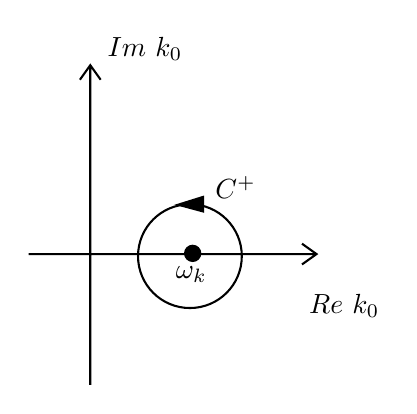
\begin{tikzpicture}[x=0.75pt,y=0.75pt,yscale=-1,xscale=1]
%uncomment if require: \path (0,300); %set diagram left start at 0, and has height of 300

%Shape: Axis 2D [id:dp7652206528593761] 
\draw  (442.67,157) -- (581.33,157)(472.33,66) -- (472.33,220) (574.33,152) -- (581.33,157) -- (574.33,162) (467.33,73) -- (472.33,66) -- (477.33,73)  ;
%Shape: Circle [id:dp9512824136083587] 
\draw   (495.33,158) .. controls (495.33,144.19) and (506.53,133) .. (520.33,133) .. controls (534.14,133) and (545.33,144.19) .. (545.33,158) .. controls (545.33,171.81) and (534.14,183) .. (520.33,183) .. controls (506.53,183) and (495.33,171.81) .. (495.33,158) -- cycle ;
%Shape: Triangle [id:dp2477537383850551] 
\draw  [fill={rgb, 255:red, 0; green, 0; blue, 0 }  ,fill opacity=1 ] (514.67,133.22) -- (526.65,129.47) -- (526.69,136.47) -- cycle ;
%Shape: Circle [id:dp6379400625529519] 
\draw  [fill={rgb, 255:red, 0; green, 0; blue, 0 }  ,fill opacity=1 ] (518,156.67) .. controls (518,154.64) and (519.64,153) .. (521.67,153) .. controls (523.69,153) and (525.33,154.64) .. (525.33,156.67) .. controls (525.33,158.69) and (523.69,160.33) .. (521.67,160.33) .. controls (519.64,160.33) and (518,158.69) .. (518,156.67) -- cycle ;

% Text Node
\draw (521,167) node    {$\omega _{k}$};
% Text Node
\draw (542.33,127) node    {$ \begin{array}{l}
C^{+}\\
\end{array}$};
% Text Node
\draw (594.67,182) node    {$Re\ k_{0}$};
% Text Node
\draw (498.67,58) node    {$Im\ k_{0}$};


\end{tikzpicture}

    \caption{Contour Integral for real, positive frequency}
    \label{fig:contour-integral-1}
\end{figure}
Now, rewrite $i\Delta^+(x-y)$ as
$$
i \Delta^{+}(x-y)=\frac{1}{(2 \pi)^{3}} \int e^{i \mathbf{k} \cdot(x-y)}\underbrace{\left\{\frac{e^{-i \omega_{k}\left(t_{x}-t_{y}\right)}}{2 \omega_{\mathbf{k}}}\right\}}_{f\left(\omega_{\mathbf{k}}\right)} d^{3} \mathbf{k}
$$
where we take the bracketed quantity as equal to $f\left(\omega_{\mathbf{k}}\right),$ and where
$$
f\left(k_{0}\right)=\frac{e^{-i k_{0}\left(t_{x}-t_{y}\right)}}{k_{0}+\omega_{\mathbf{k}}}
$$
We can then use $f(k_0)$ to find
\begin{equation}
\begin{aligned}
i \Delta^{+}(x-y) &=\frac{1}{(2 \pi)^{3}} \int e^{i \mathbf{k} \cdot(x-y)}\left\{\frac{1}{i 2 \pi} \int_{C^{+}} \frac{f\left(k_{0}\right)}{k_{0}-\omega_{\mathbf{k}}} d k_{0}\right\} d^{3} \mathbf{k} \\
&=\frac{1}{(2 \pi)^{3}} \int e^{i \mathbf{k} \cdot(x-y)}\left\{\frac{1}{i 2 \pi} \int_{C^{+}} \frac{e^{-i k_{0}\left(t_{x}-t_{y}\right)}}{\left(k_{0}-\omega_{\mathbf{k}}\right)\left(k_{0}+\omega_{\mathbf{k}}\right)} d k_{0}\right\} d^{3} \mathbf{k} \\
&=\frac{-i}{(2 \pi)^{4}} \int_{C^+} \frac{e^{-i k(x-y)}}{\left(k_{0}\right)^{2}-\left(\omega_{\mathbf{k}}\right)^{2}} d^{4} k
\end{aligned}
\end{equation}
where the integral notation now implies integration over four dimensions of the 4 -momentum, with the 3 -momentum part from $-\infty$ to $+\infty$ in real space and the energy part a contour integral in complex space. Note that the integral does not "blow up" because $k_{0} \neq \omega_{\mathrm{k}}$ over the contour integral. \textbf{$k_0$ has at this point become, for us, a variable that generally does not equal energy $\omega_{\mathbf{k}}$}.

Because the following relations are always true for any four vector,
\begin{equation}
k^{2}=\left(k_{0}\right)^{2}-(\mathbf{k})^{2} \rightarrow\left(k_{0}\right)^{2}=k^{2}+(\mathbf{k})^{2}
\end{equation}
we have
\begin{equation}
a_{k}^{2}-(k)^{2}=\mu^{2} \quad \rightarrow \quad \omega_{k}^{2}=\mu^{2}+(k)^{2}
\end{equation}
and thus,
\begin{equation}
i \Delta^{+}(x-y)=\frac{-i}{(2 \pi)^{4}} \int_{C^{+}} \frac{e^{-i k(x-y)}}{k^{2}-\mu^{2}} d^{4} k
\end{equation}
For $i \Delta^{-}(x-y),$ we carry out similar steps except that the contour integral (still counter clock-wise [ccw], as in Fig. \ref{fig:contour-integral-1}) is now about $-\omega_{\mathbf{k}} .$ When all is said and done, we find the only differences to be the sign and the contour, which is now about the negative frequency value and designated by $C^-$:
\begin{equation}
i \Delta^{-}(x-y)=\frac{i}{(2 \pi)^{4}} \int_{C^{-}} \frac{e^{-i k(x-y)}}{k^{2}-\mu^{2}} d^{4} k
\end{equation}
\underline{\textbf{We then re-express $i\Delta_F$ in most convenient form using the contour shown below:}}
\begin{figure}[H]
    \centering
    


\tikzset{every picture/.style={line width=0.75pt}} %set default line width to 0.75pt        

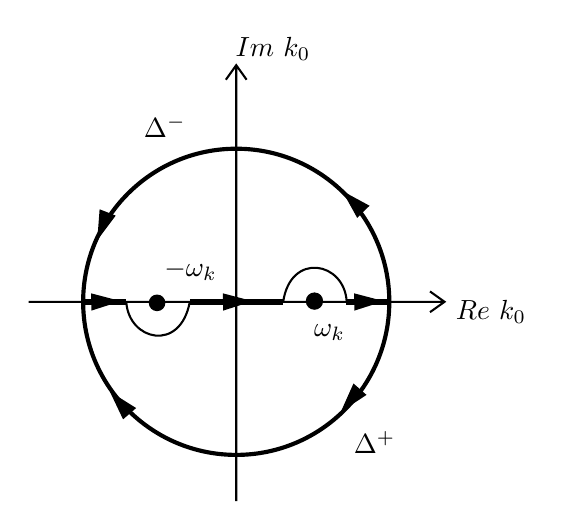
\begin{tikzpicture}[x=0.75pt,y=0.75pt,yscale=-1,xscale=1]
%uncomment if require: \path (0,300); %set diagram left start at 0, and has height of 300

%Shape: Axis 2D [id:dp7652206528593761] 
\draw  (381,180) -- (581.33,180)(480.98,66) -- (480.98,276) (574.33,175) -- (581.33,180) -- (574.33,185) (475.98,73) -- (480.98,66) -- (485.98,73)  ;
%Shape: Circle [id:dp9512824136083587] 
\draw  [line width=1.5]  (407.22,180) .. controls (407.22,139.27) and (440.24,106.24) .. (480.98,106.24) .. controls (521.71,106.24) and (554.73,139.27) .. (554.73,180) .. controls (554.73,220.73) and (521.71,253.76) .. (480.98,253.76) .. controls (440.24,253.76) and (407.22,220.73) .. (407.22,180) -- cycle ;
%Shape: Triangle [id:dp2477537383850551] 
\draw  [fill={rgb, 255:red, 0; green, 0; blue, 0 }  ,fill opacity=1 ] (533.33,127.84) -- (544.37,133.83) -- (539.37,138.73) -- cycle ;
%Shape: Circle [id:dp6379400625529519] 
\draw  [fill={rgb, 255:red, 0; green, 0; blue, 0 }  ,fill opacity=1 ] (515,179.67) .. controls (515,177.64) and (516.64,176) .. (518.67,176) .. controls (520.69,176) and (522.33,177.64) .. (522.33,179.67) .. controls (522.33,181.69) and (520.69,183.33) .. (518.67,183.33) .. controls (516.64,183.33) and (515,181.69) .. (515,179.67) -- cycle ;
%Shape: Triangle [id:dp23597183881740225] 
\draw  [fill={rgb, 255:red, 0; green, 0; blue, 0 }  ,fill opacity=1 ] (414.65,148.65) -- (415.6,136.14) -- (422.12,138.69) -- cycle ;
%Straight Lines [id:da962016249657206] 
\draw [line width=2.25]    (407.22,180) -- (428,180) ;


%Straight Lines [id:da7964252184040902] 
\draw [line width=2.25]    (533.95,180) -- (554.73,180) ;


%Curve Lines [id:da28222125380035745] 
\draw    (503.6,180) .. controls (507.2,155.67) and (533.2,160.67) .. (534.2,180) ;


%Shape: Circle [id:dp990916237206093] 
\draw  [fill={rgb, 255:red, 0; green, 0; blue, 0 }  ,fill opacity=1 ] (439.33,180.5) .. controls (439.33,178.57) and (440.9,177) .. (442.83,177) .. controls (444.77,177) and (446.33,178.57) .. (446.33,180.5) .. controls (446.33,182.43) and (444.77,184) .. (442.83,184) .. controls (440.9,184) and (439.33,182.43) .. (439.33,180.5) -- cycle ;
%Straight Lines [id:da4611299798430879] 
\draw [line width=2.25]    (458.6,180) -- (503.6,180) ;


%Curve Lines [id:da707145238278245] 
\draw    (428,180) .. controls (429.1,198.67) and (454.1,204.67) .. (458.6,180) ;


%Shape: Triangle [id:dp0397944332871496] 
\draw  [fill={rgb, 255:red, 0; green, 0; blue, 0 }  ,fill opacity=1 ] (423.61,179.74) -- (411.65,183.57) -- (411.57,176.57) -- cycle ;
%Shape: Triangle [id:dp33828685579909257] 
\draw  [fill={rgb, 255:red, 0; green, 0; blue, 0 }  ,fill opacity=1 ] (487.1,179.74) -- (475.14,183.57) -- (475.06,176.57) -- cycle ;
%Shape: Triangle [id:dp330061649893429] 
\draw  [fill={rgb, 255:red, 0; green, 0; blue, 0 }  ,fill opacity=1 ] (550.34,179.74) -- (538.38,183.57) -- (538.3,176.57) -- cycle ;
%Shape: Triangle [id:dp8172867825474798] 
\draw  [fill={rgb, 255:red, 0; green, 0; blue, 0 }  ,fill opacity=1 ] (532.53,231.64) -- (537.65,220.18) -- (542.92,224.79) -- cycle ;
%Shape: Triangle [id:dp6169947743207842] 
\draw  [fill={rgb, 255:red, 0; green, 0; blue, 0 }  ,fill opacity=1 ] (421.28,224.58) -- (431.91,231.25) -- (426.62,235.83) -- cycle ;

% Text Node
\draw (526,195) node    {$\omega _{k}$};
% Text Node
\draw (603.67,185) node    {$Re\ k_{0}$};
% Text Node
\draw (498.67,58) node    {$Im\ k_{0}$};
% Text Node
\draw (459,165) node    {$-\omega _{k}$};
% Text Node
\draw (446.6,95.67) node    {$\Delta ^{-}$};
% Text Node
\draw (547.6,247.67) node    {$\Delta ^{+}$};


\end{tikzpicture}

    \caption{Contour integrals for $\Delta^{\pm}$}
    \label{fig:delta-pm-contour}
\end{figure}
The lower loop shown above encloses $+\omega_{\mathrm{k}},$ but since it has a cw integration path, the result will have a sign change, and hence equals the ccw integration. Thus, the lower loop represents $\Delta^{+}$. This means we can define the Feynman propagator as \textbf{proportional to the same integral over the two different loops.} We say proportional because we also have to include the concomitant integration over the 3D space of $\mathbf{k}$. So we can then re-write the Feynman propagator as:
\begin{equation}
i \Delta_{F}(x-y)=\frac{i}{(2 \pi)^{4}} \int_{C_{F}} \frac{e^{-i k(x-y)}}{k^{2}-\mu^{2}} d^{4} k
\label{convenient-delta-F}
\end{equation}
where $C_F$ is the contour shown in Fig.\ref{fig:delta-pm-contour}.

Now, consider enlarging the outer hemispheric parts of the two loops, so they extend essentially to infinity. The value of the contour integrals over them will remain unchanged. But the $k^2$ value in the denominator of (\ref{convenient-delta-F}) will become so large that any contribution to the integral over those parts of the path will become negligible.

We can further simplify by \textbf{moving the poles an infinitesimal distance $\eta$ of the real axis} as shown in the figure below and deform the contour so that it is all along the real axis.In the limit as $\eta\rightarrow0$, the integral will have the same value, though we must now include this slight pole shift in the propagator expression (\ref{convenient-delta-F}).
\begin{figure}[H]
    \centering

\tikzset{every picture/.style={line width=0.75pt}} %set default line width to 0.75pt        

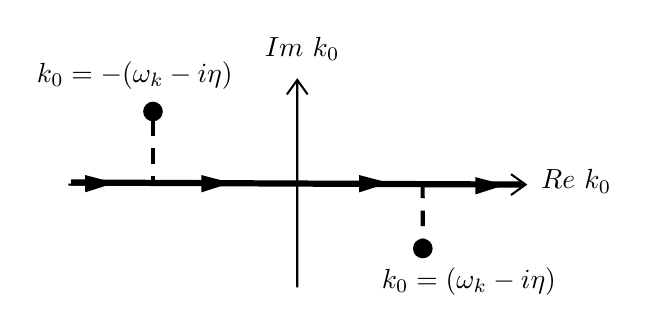
\begin{tikzpicture}[x=0.75pt,y=0.75pt,yscale=-1,xscale=1]
%uncomment if require: \path (0,300); %set diagram left start at 0, and has height of 300

%Shape: Axis 2D [id:dp7920230309283391] 
\draw  (50,174.53) -- (270.3,174.53)(160.3,124.1) -- (160.3,224.1) (263.3,169.53) -- (270.3,174.53) -- (263.3,179.53) (155.3,131.1) -- (160.3,124.1) -- (165.3,131.1)  ;
%Straight Lines [id:da7847785231808648] 
\draw [line width=2.25]    (51.3,173.53) -- (268.3,174.53) ;


%Shape: Triangle [id:dp1487065899952008] 
\draw  [fill={rgb, 255:red, 0; green, 0; blue, 0 }  ,fill opacity=1 ] (70.61,173.74) -- (58.65,177.57) -- (58.57,170.57) -- cycle ;
%Shape: Triangle [id:dp7913173487008308] 
\draw  [fill={rgb, 255:red, 0; green, 0; blue, 0 }  ,fill opacity=1 ] (126.61,173.74) -- (114.65,177.57) -- (114.57,170.57) -- cycle ;
%Shape: Triangle [id:dp49881933214308327] 
\draw  [fill={rgb, 255:red, 0; green, 0; blue, 0 }  ,fill opacity=1 ] (202.61,173.74) -- (190.65,177.57) -- (190.57,170.57) -- cycle ;
%Shape: Triangle [id:dp5855067458502727] 
\draw  [fill={rgb, 255:red, 0; green, 0; blue, 0 }  ,fill opacity=1 ] (258.61,174.74) -- (246.65,178.57) -- (246.57,171.57) -- cycle ;
%Shape: Circle [id:dp9429340464530463] 
\draw  [fill={rgb, 255:red, 0; green, 0; blue, 0 }  ,fill opacity=1 ] (86.57,139.32) .. controls (86.57,136.99) and (88.45,135.1) .. (90.78,135.1) .. controls (93.11,135.1) and (95,136.99) .. (95,139.32) .. controls (95,141.65) and (93.11,143.53) .. (90.78,143.53) .. controls (88.45,143.53) and (86.57,141.65) .. (86.57,139.32) -- cycle ;
%Straight Lines [id:da10788367472784177] 
\draw [line width=1.5]  [dash pattern={on 5.63pt off 4.5pt}]  (90.78,143.53) -- (90.78,174.53) ;


%Shape: Circle [id:dp24532399791813508] 
\draw  [fill={rgb, 255:red, 0; green, 0; blue, 0 }  ,fill opacity=1 ] (216.57,205.32) .. controls (216.57,202.99) and (218.45,201.1) .. (220.78,201.1) .. controls (223.11,201.1) and (225,202.99) .. (225,205.32) .. controls (225,207.65) and (223.11,209.53) .. (220.78,209.53) .. controls (218.45,209.53) and (216.57,207.65) .. (216.57,205.32) -- cycle ;
%Straight Lines [id:da12412627922403063] 
\draw [line width=1.5]  [dash pattern={on 5.63pt off 4.5pt}]  (220.7,173.53) -- (220.78,201.1) ;



% Text Node
\draw (294.67,173) node    {$Re\ k_{0}$};
% Text Node
\draw (162.67,109) node    {$Im\ k_{0}$};
% Text Node
\draw (82,122.1) node    {$k_{0} =-( \omega _{k} -i\eta )$};
% Text Node
\draw (243,221.1) node    {$k_{0} =( \omega _{k} -i\eta )$};


\end{tikzpicture}

    \caption{Contour and displaced poles for $\Delta_F$}
    \label{fig:displaced-pole}
\end{figure}
Again, with $k^{2}-\mu^{2}=\left(k_{0}\right)^{2}-\left(\omega_{\mathbf{k}}\right)^{2}$, we have
$$
i \Delta_{F}(x-y)=\frac{i}{(2 \pi)^{4}} \int_{-\infty}^{+\infty} \frac{e^{-i k(x-y)}}{\left(k_{0}\right)^{2}-\left(\omega_{\mathbf{k}}-i \eta\right)^{2}} d^{4} k
$$
If we use $k^{2}-\mu^{2}=\left(k_{0}\right)^{2}-\left(\omega_{\mathbf{k}}\right)^{2}$ again, and take $\epsilon=2\eta\omega_{\mathbf{k}}$, we have our \textbf{final result for the Feynman scalar propagator}:
\begin{qt}
    \begin{equation}
i \Delta_{F}(x-y)=\frac{i}{(2 \pi)^{4}} \int_{-\infty}^{+\infty} \frac{e^{-i k(x-y)}}{k^{2}-\mu^{2}+i \varepsilon} d^{4} k
\label{Feynman-scalar-propagator-final}
\end{equation}
\end{qt}
From (\ref{Feynman-scalar-propagator-final}), we can readily write down \textbf{the 4-momentum space form of the propagator},\textbf{the Fourier transform of (\ref{Feynman-scalar-propagator-final})}, which is
\begin{qt}
    \begin{equation}
\Delta_{F}(k)=\frac{1}{k^{2}-\mu^{2}+i \varepsilon}
\end{equation}
\end{qt}